\documentclass{article}
\usepackage[utf8]{inputenc}
\usepackage{amssymb,
  amsmath,hyperref,verbatim,listings,graphicx,subfigure,fullpage, braket}
\renewcommand\vec[1]{\ensuremath{\mathbf{#1}}}

\begin{document}

\title{UML computer project 2}
\author{
Juha-Antti Isojärvi\\
013455341 \\
Department of Mathematics and Statistics\\
Master student
\and
Mikko Sysikaski\\
013573016\\
Department of Computer Science\\
Master student}
\date{}
\maketitle

\section{Exercise set 1}
In the first set of exercise we compared results of applying ICA to
uniformly distributed and gaussian data.
\subsection{Exercise 1}\label{sec:11}
First we needed some data. We were given two mixing matrices 
\[
A_1 = \left[ \begin{array}{ccc}
0.4483 & -1.6730  \\
2.1907 & -1.4836  \end{array} \right], \quad
A_2 = \left[ \begin{array}{ccc}
0 & -1.7321  \\
1.7321 & -2.0  \end{array} \right].
\]
These matrices were then used to mix a sample \textbf{s} of uniformly distributed
data and a sample \textbf{n} of gaussian data, each containing 5000
points. The results of mixing are denoted 
\[
\begin{array}{ccc}
\textbf{x}_1 = A_1\textbf{s}, \\
\textbf{x}_2 = A_2\textbf{s}, \\
\textbf{y}_1 = A_1\textbf{n}, & \textup{and} \\
\textbf{y}_2 = A_2\textbf{n}.
\end{array}
\]

Scatter plots of the original and mixed data can be seen in figure
\ref{fig:scatterE21}. In our previous report we described how standard
normally distributed data with zero mean and covariance $\Sigma$ has a
multinormal distribution with zero mean and covariance $AA^T$, after
it is linearly transformed with a matrix $A$. Thus 
\[
E \textbf{y}_1 = 0 = E \textbf{y}_2,
\]
and 
\[
\textup{cov}(\textbf{y}_1) = A_1A_1^T = \left[ \begin{array}{ccc}
3.000 & 3.4642  \\
3.4642 & 7.000  \end{array} \right], \quad
\textup{cov}(\textbf{y}_1) = A_1A_1^T = \left[ \begin{array}{ccc}
3.000 & 3.4642  \\
3.4642 & 7.000  \end{array} \right].
\] 
Notice that though the mixing matrices are different, the covariance
of the mixed data is equal. Below the computed sample covariance and mean of the mixed data:
\begin{verbatim}
> mean(y1)
[1] -0.007008821
> mean(y2)
[1] -0.01386588
> cov(y1)
         [,1]     [,2]
[1,] 2.898259 3.317027
[2,] 3.317027 6.749532
> cov(y2)
         [,1]     [,2]
[1,] 2.917094 3.328705
[2,] 3.328705 6.733001
\end{verbatim}
As can be seen, the sample covariance and mean are roughly equal to the covariance and mean of the
underlying distribution, as is expected.

\begin{figure}\centering
	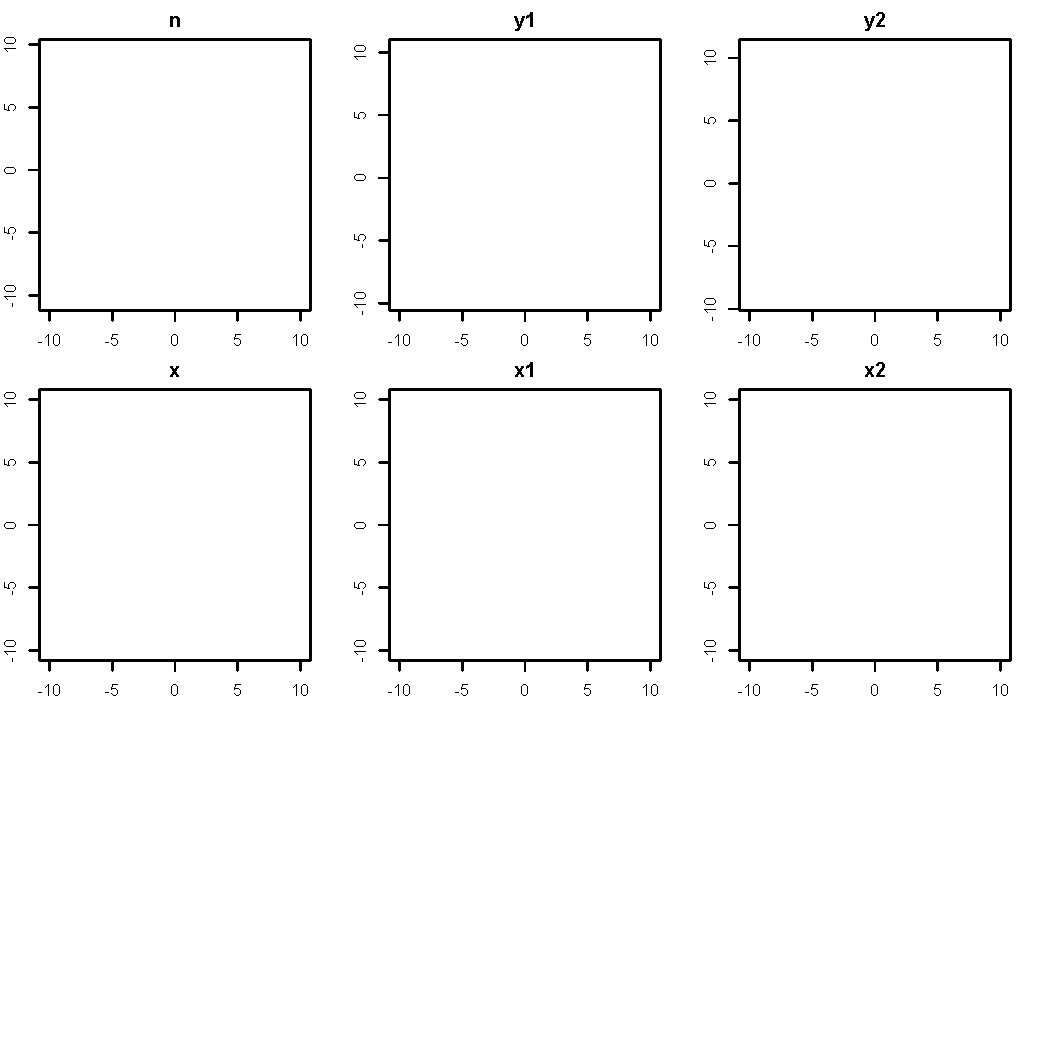
\includegraphics[trim = 0cm 5.9cm 0cm 0cm, clip = true,
totalheight=0.5\textheight]{scatterPlotE21.pdf}
	\caption{Scatter plots of the data before and after
          mixing. The first column shows the unmixed data, the second column
          the data mixed with $A_1$ and the third the data mixed with $A_2$.} \label{fig:scatterE21}
\end{figure}

\subsection{Exercise 2}
Now that we had our generated artificial data, the first step of ICA
is to whiten the data. The results of applying the PCA based whitening
transformation can be seen plotted in figure \ref{fig:scatterWhiteE22}.
The whitening matrices used were:
\begin{verbatim}
> whiteningY1
           PC1        PC2
[1,] 0.1695626  0.2945006
[2,] 0.8716748 -0.5018783
> whiteningY2
          PC1        PC2
[1,] 0.170350  0.2939907
[2,] 0.870344 -0.5043123
> whiteningX1
           PC1        PC2
[1,] 0.1639257  0.2850347
[2,] 0.8680057 -0.4991970
> whiteningX2
            PC1        PC2
[1,] -0.1635482 -0.2860464
[2,] -0.8673773  0.4959264
\end{verbatim}
We failed to see the connection between the whitening matrices and the
mixing matrices.
% PCA:
% \begin{verbatim}
% > prcomp(y1)
% Standard deviations:
% [1] 2.9426781 0.9942015

% Rotation:
%            PC1        PC2
% [1,] 0.4989681  0.8666204
% [2,] 0.8666204 -0.4989681
% > prcomp(y2)
% Standard deviations:
% [1] 2.9430913 0.9941372

% Rotation:
%            PC1        PC2
% [1,] 0.5013556  0.8652413
% [2,] 0.8652413 -0.5013556
% > prcomp(x1)
% Standard deviations:
% [1] 3.0412644 0.9986868

% Rotation:
%            PC1        PC2
% [1,] 0.4985415  0.8668658
% [2,] 0.8668658 -0.4985415
% > prcomp(x2)
% Standard deviations:
% [1] 3.034897 1.000858

% Rotation:
%             PC1        PC2
% [1,] -0.4963519 -0.8681214
% [2,] -0.8681214  0.4963519
%\end{verbatim}
\begin{figure}\centering
	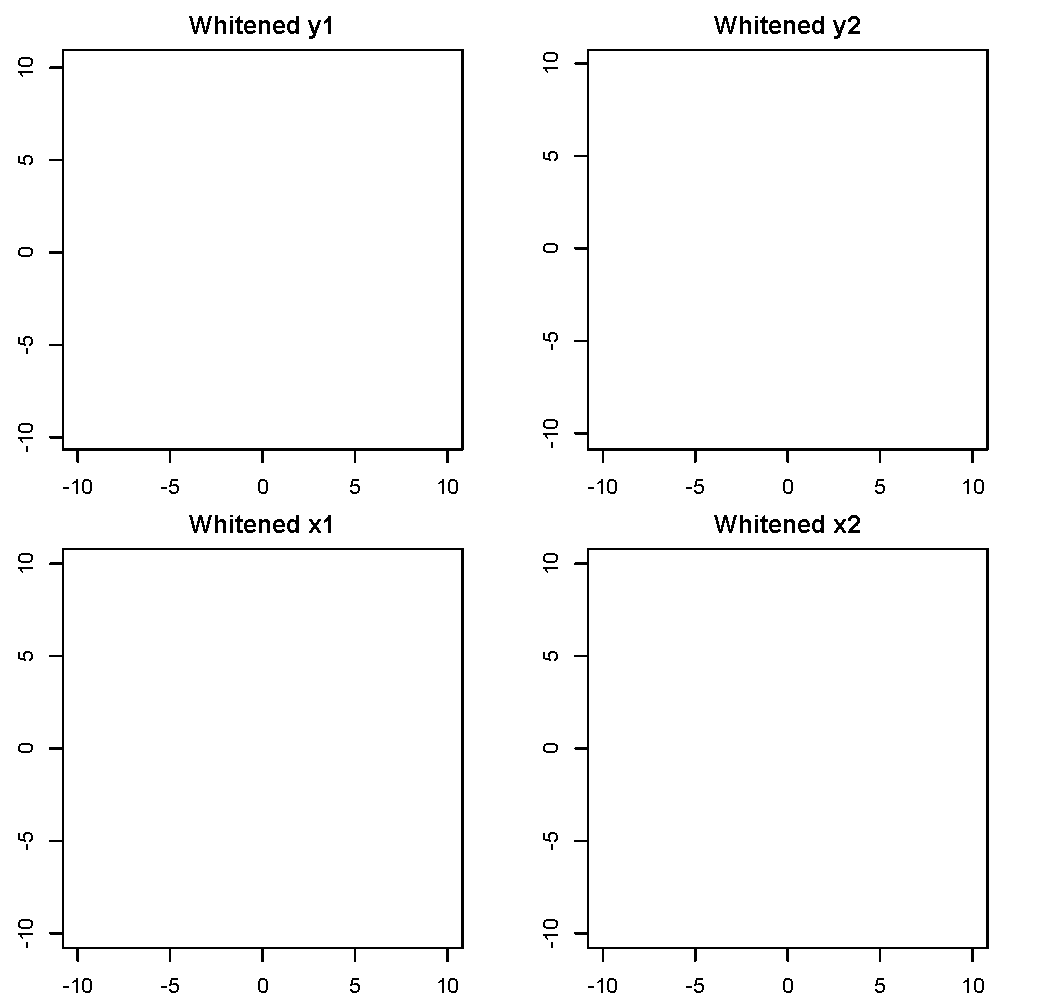
\includegraphics[totalheight=0.5\textheight]{scatterPlotOfWhitenedE22.pdf}
	\caption{Scatter plots of the whitened data.} \label{fig:scatterWhiteE22}
\end{figure}

\subsection{Exercise 3}
ICA can be solved by maximizing kurtosis. In figure
\ref{fig:kurtosisAlphaE23} the kurtosis of each mixed whitened
data, projected onto a unit vector \textbf{w} which forms an angle
$\alpha \in [0,\pi]$ with the $x$-axis, is plotted as a function of
alpha. 

The plots show larger absolute values of kurtosis for the uniform data, as for
the gaussian data. Also, the kurtosis of the uniform distribution is a
sine curve, which is fairly regular as should be expected for
nongaussian ICs. Coincidentally, the gaussian distribution also show a
sine-like curve for kurtosis. In repeated further tests the kurtosis
of the gaussian data showed more irregularity. In fact the gaussian
data should have kurtosis of zero, and different values of kurtosis
are the result of chance.

Kurtosis was maximized for the following $\alpha$:
\begin{verbatim}
> maxAlphaY1
[1] 1.006316
> maxAlphaY2
[1] 0.7390133
> maxAlphaX1
[1] 0.7798949
> maxAlphaX2
[1] 0.5220264
\end{verbatim}
\begin{figure}\centering
	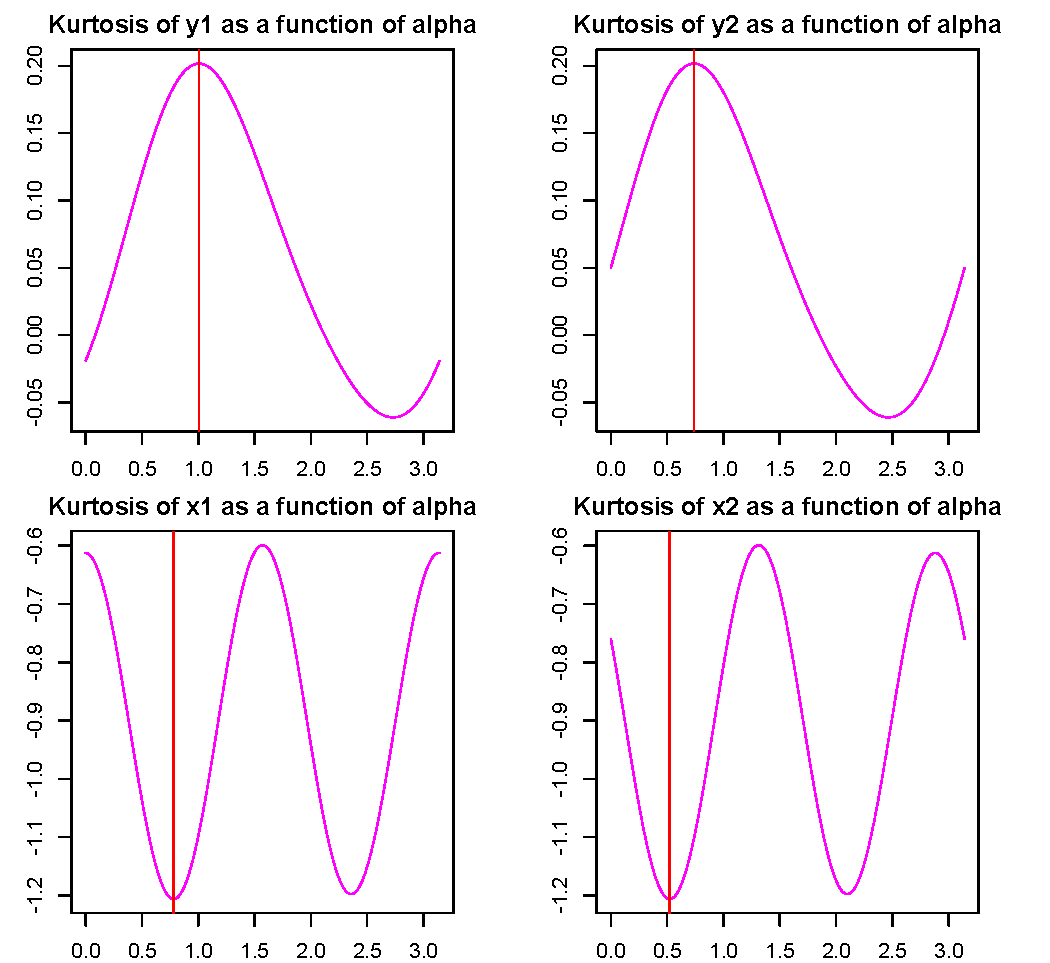
\includegraphics[totalheight=0.5\textheight]{kurtosisAlphaE23.pdf}
	\caption{Kurtosis as a function of alpha.} \label{fig:kurtosisAlphaE23}
\end{figure}
\subsection{Exercise 4}
The optimal projection vectors $\textbf{b}_i$ are the rows of the inverse of the
whitened matrix $A_w$
\[
B = \left[ \begin{array}{ccc}
b_1^T  \\
b_2 ^T \end{array} \right] = A_w^{-1}.
\]
$A_w$ is the result of transforming the original $A$ with the
whitening matrix denoted here by $W$:
\[
A_w = WA.
\]
Therefore $A$ can be estimated using the whitening matrix and the optimal
vectors in the following manner:
\[
A = W^-1B^-1.
\]
Our estimates are shown below:
\begin{verbatim}
> estA(x1,1000)
          [,1]     [,2]
[1,] 0.4213442 1.672819
[2,] 2.1730399 1.504597
> A1
       [,1]    [,2]
[1,] 0.4483 -1.6730
[2,] 2.1907 -1.4836
> estA(x2,1000)
            [,1]     [,2]
[1,] -0.02973494 1.726432
[2,]  1.70379490 2.014105
> A2
       [,1]    [,2]
[1,] 0.0000 -1.7321
[2,] 1.7321 -2.0000
> estA(y1,1000)
          [,1]       [,2]
[1,] -1.373120  1.0530153
[2,] -2.634125 -0.1839215
> A1
       [,1]    [,2]
[1,] 0.4483 -1.6730
[2,] 2.1907 -1.4836
> estA(y2,1000)
          [,1]     [,2]
[1,] -1.054454 1.379936
[2,] -2.586195 0.514233
> A2
       [,1]    [,2]
[1,] 0.0000 -1.7321
[2,] 1.7321 -2.0000
\end{verbatim}
Notice that the uniform data gives good estimates for the mixing
matrices, whereas the gaussian data gives bad estimates.
\subsection{Exercise 5}
Exercise 5 was to explain the above result: why is it possible to find
an estimate for $A_1$ and $A_2$ for the uniform data, but not for the
gaussian data?

The reason for this is that the whitened matrix $A_w$ is orthogonal,
and therefore, if \textbf{s} is gaussian, $A_ws$ is also gaussian and
white. Now there is no unique solution to the optimal projection
$b_i^TA_ws$, because of orthogonality assumption for the estimated ICs
$b_i$.




\section{Exercise set 2}
Next we were given the task of performing ICA on 32 independent
variables following a Laplacian distribution with zero mean and unit variance.

\subsection{Exercise 1}
First we needed to artificially generate the data. We achieved this by
first drawing a sample $u$ of 10000 points from a uniform distribution on
the interval $[-0.5 \; 0.5]$, and then transforming the data by $s =
1/\sqrt(2) \cdot \textup{sign}(u) \cdot \log(1-2|u|)$. Such a variable
\textbf{s} then follows a Laplacian distribution with zero mean and
unit variance. Repeating this generation process 32 times creates a
sample of 10000 points of a random vector which consists of 32 independent random
variables following the desired Laplacian distribution.

Next the generated data was transformed by summing the $m$ first $s_i$
and then normalizing to unit variance. The result
\[ \tilde{y}_m = \sum_{i = 1}^m s_i \quad \textrm{and} \quad y_m =
\frac{\tilde{y}_m}{\sqrt{\textup{Var}(\tilde{y}_m)}}.
\]

Then we computed an estimate for the pdf's of the variables $y_m$, $m
\in \set{1,2,4,8,16,32}$. We approached this in two ways, by using a
histogram estimation, and by using the kernel density estimation
method implemented in R. Only the results of the latter will be shown
here, as the purpose was only to illustrate the similarity of the log
density of the normalized sums to the similarity of the gaussian log
density.

The logarithm densities of the six variables can be seen in figure
\ref{fig:logDensE221}.  Notice how the two densities become more
similar, as $m$ grows. This is of course explained by the central
limit theorem.

\begin{figure}\centering
	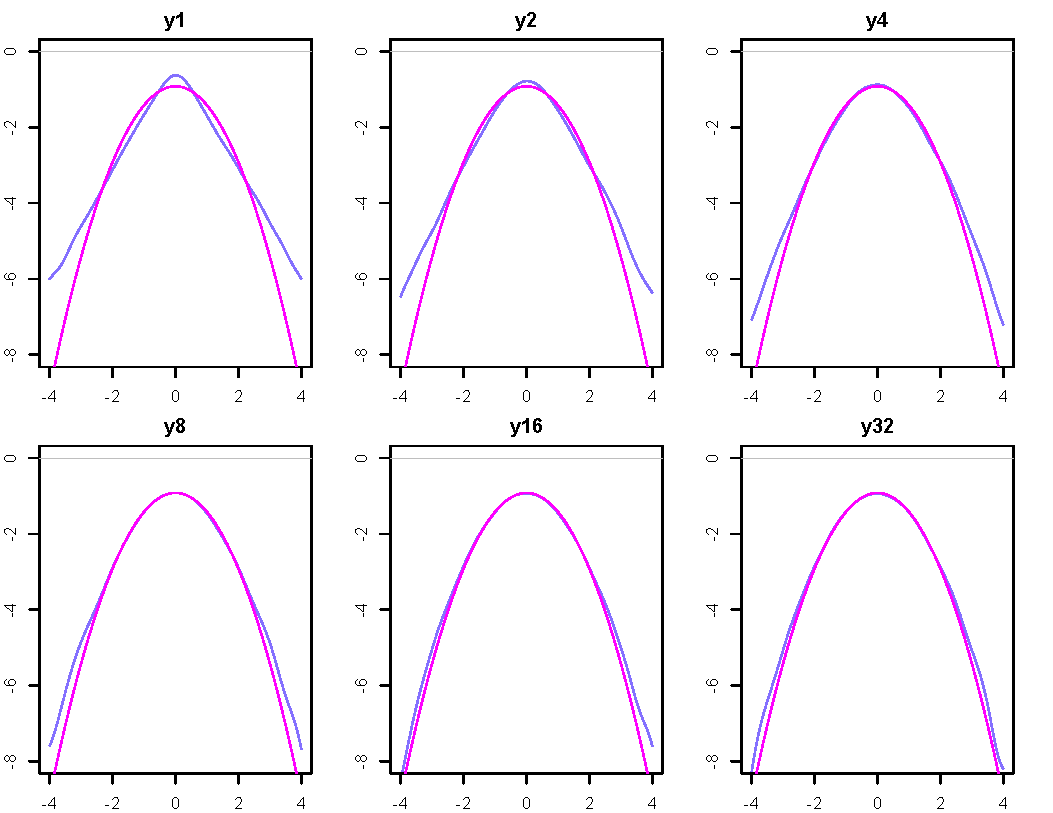
\includegraphics[totalheight=0.5\textheight]{logDensE221.pdf}
	\caption{The logartihm densities for variables $y_m$, $m \in
          \set{1,2,4,8,16,32}$ in magenta, and the gaussian logarithm density
          in blue.} \label{fig:logDensE221}
\end{figure}

\subsection{Exercise 2}
As was seen in the previous exercise, the variables $y_m$ tend to the
gaussian distribution. If kurtosis is a good measure of gaussianity,
this would also imply, that the kurtosis of $y_m$ should tend to
zero. The kurtosis of $y_m$ as a function of $m$ can be seen plotted
in figure \ref{fig:kurtosisM}.

\begin{figure}\centering
	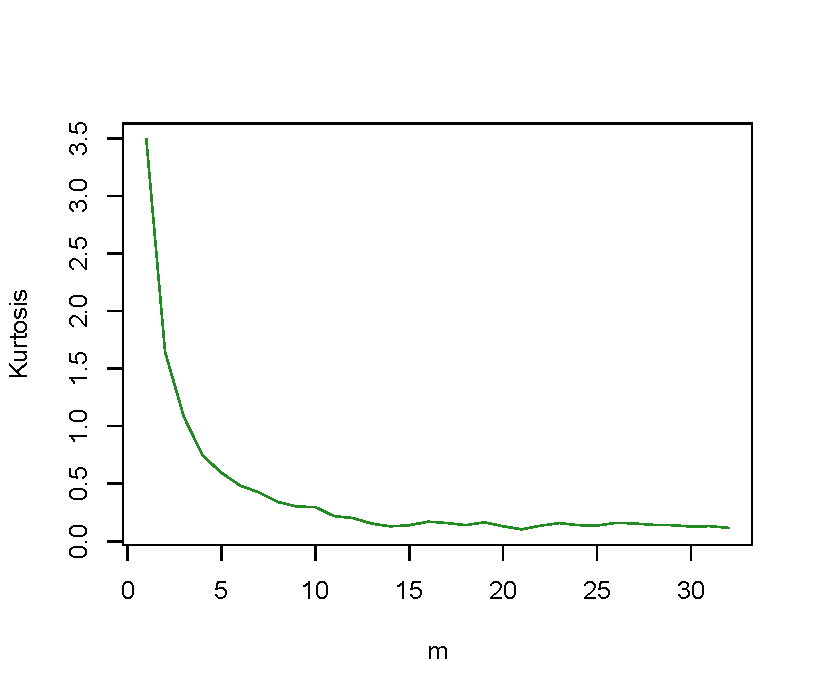
\includegraphics[trim = 0cm 0.5cm 0cm 1cm, clip = true, totalheight=0.5\textheight]{kurtosisM.pdf}
	\caption{The kurtosis of $y_m$ as a function of $m$.} \label{fig:kurtosisM}
\end{figure}

\subsection{Exercise 3}
In this exercise we were given the task to implement the ICA algorithm
based on symmetric orthogonalization. For the one unit algorithm we
both used the fast fixed point algorithm. As a stop criterion one could use
the difference between the kurtoses after each iteration.

We tested our implementations on the uniform data set of Exercise set
1 transformed with matrix $A1$. The result can be seen below
\begin{verbatim}
> A1
       [,1]    [,2]
[1,] 0.4483 -1.6730
[2,] 2.1907 -1.4836
> estA1
          [,1]     [,2]
[1,] 0.4367542 1.690438
[2,] 2.1952565 1.542458
\end{verbatim}
Notice that the estimate is very close to the original, with ambiguity
of sing in the second column.

\subsection{Exercise 4}
The matrix transforming $\textbf{s} \to \tilde{\textbf{y}}$, $y_m = \sum_{i=1}^m s_i$, is given by
the lower triangular matrix of which every nonzero element is equal to
one. An example in three dimensions:
\[
\Sigma =
\left[ \begin{array}{ccc}
1 & 0 & 0 \\
1 & 1 & 0 \\
1 & 1 & 1 \end{array} \right],
\quad
\tilde{\textbf{y}} = \Sigma \textbf{s} = (s_1, s_1 + s_2, s_1 + s_2 + s_3)^T.
\]
To normalize $y_m$, the variance is required. After estimating
the variance, the transformation $\tilde{\textbf{y}} \to \textbf{y}$
is achieved via multiplication by the diagonal matrix $D$ containing the
standard deviations: 
\[
\textbf{y} = D \tilde{\textbf{y}}= \textup{diag} \left( \frac{1}{\sqrt{\textup{var}(y_i)}}
\right) \tilde{\textbf{y}}.
\]

Now, after transforming $\textbf{s} \to \tilde{\textbf{y}}$ and
estimating the variance, one gets matrices $D$ and $\Sigma$. Their
product $A = D \Sigma$ gives the transformation matrix $\textbf{s} \to
\textbf{y}$:
\[
\textbf{y} = A\textbf{s}.
\]
\subsection{Exercise 5}
In this exercise we estimated the mixing matrix $A$ from the previous
exercise by using the ICA algorithm we implemented in exercise 3. The
average squared error of the estimate of $A$ with 10000 points and
20000 points can be seen below. 
10000 points:
\begin{verbatim}
> mean(1/32^2 * (Ahat-A)^2)
[1] 6.775627e-05
\end{verbatim}
20000 points:
\begin{verbatim}
> mean(1/32^2 * (Ahat-A)^2)
[1] 5.675457e-05
\end{verbatim}
These show no significant change, although the change is in the right
direction of smaller error for more points. 

\section{Exercise set 3}

\subsection{Exercise 1}

In the third exercise we were given six images which were weighted sums of six hidden source images, and the goal was to recover the original images from the mixtures.
The visualization of the mixed images is shown in Figure~\ref{fig:mixed}. The images were given as a data matrix $X\in\mathbb{R}^{6\times 90000}$ where each row represents a $300\times 300$ image.

For a single image, we can assume that each pixel is a sample of a random variable with distribution defined by the color distribution of the image.
In order to apply the ICA model we have to assume that the random variables are independent of each other.
Since the source images are unrelated to each other the pixels of different source images at the same position are not directly correlated.
However, since the pixel values are not truly random, there are usually some hidden depencies between real world images.
For instance, suppose that $s_1$ and $s_2$ are two source images and $p$ and $q$ are pixel positions.
If $(s_1)_p\approx(s_1)_q$, then $p$ and $q$ are more likely to be close to each other in the images than if the values are very different, and thus $(s_2)_p$ and $(s_2)_q$ are also likely to be quite close to each other.
In practice this correlation appears to be small enough that we can still separate a small number of images quite well.

\newcommand\iscale{0.45}
\begin{figure}\centering
	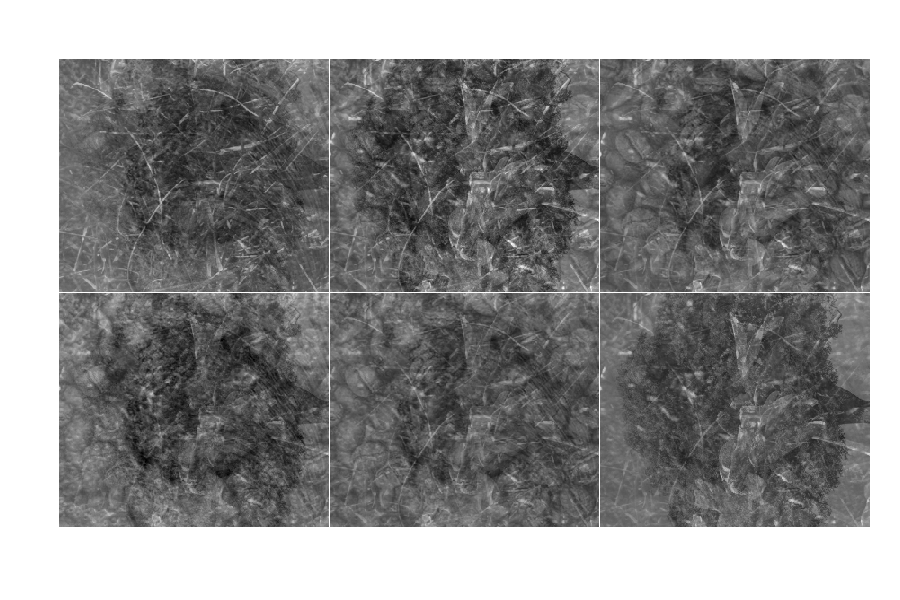
\includegraphics[scale=\iscale]{mixed}
	\caption{Mixed images used as a source of ICA.}\label{fig:mixed}
\end{figure}

\subsection{Exercise 2}
Whitening transforms the random variables into uncorrelated ones.
This is partially what we want to do in ICA, as independent variables are also uncorrelated.
Each of the image data vectors was already centered around 0, so the data could be whitened with a simple linear transform obtained from the primary components of the data.
The result of performing the whitening transform is shown in Figure~\ref{fig:white}.
The images are still quite hard to recognize, but the whitening makes some features appear in some images more clearly than in others.

\begin{figure}\centering
	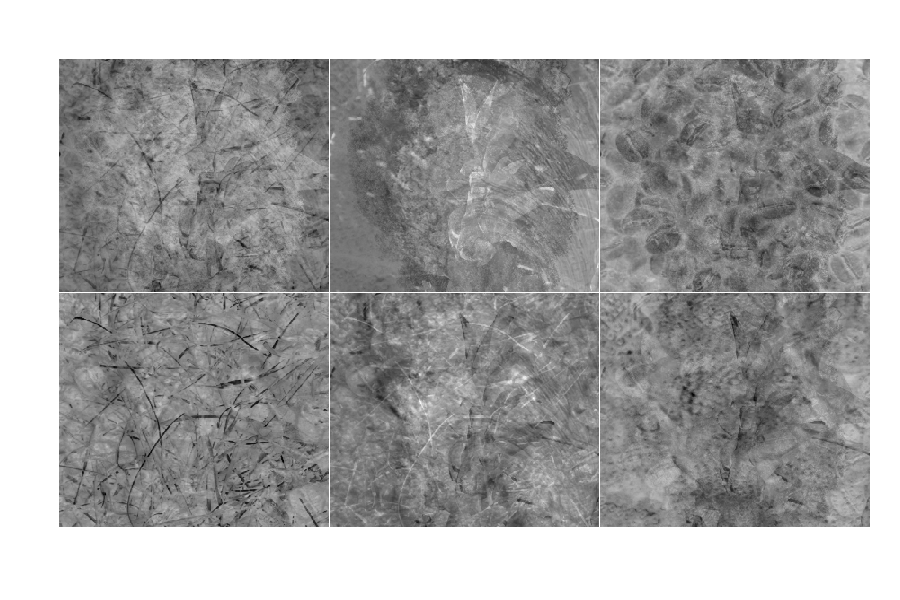
\includegraphics[scale=\iscale]{white}
	\caption{Result of doing a whitening transform for the images of Figure~\ref{fig:mixed}.}\label{fig:white}
\end{figure}

\subsection{Exercise 3}
We implemented the maximum likelihood based gradient descend ICA algorithm described in the exercise.
The algorithm maintains variables $\gamma_i$ which estimate the types of variables such that $\gamma_i$ is positive if the $i$th variable is supergaussian and negative if the variable is subgaussian.
The algorithm constructs a matrix $B\in\mathbb{R}^{n\times n}$ from the whitened random vector $\vec z\in\mathbb{R}^n$ such that $\vec y=B\vec z$ consists of the estimated latent variables.
The convergence of objective $F=-\sum_i\gamma_iE(\log\cosh(y_i))$ is used to measure when the algorithm has converged.

The algorithm was tested on the point set \vec{x_1} defined in Section~\ref{sec:11}.
The Figure~\ref{fig:icatest} shows that the original uniformly distributed random variables were succesfully recovered.
The figure also shows the progress of the objective function during the gradient descend.

\begin{figure}\centering
	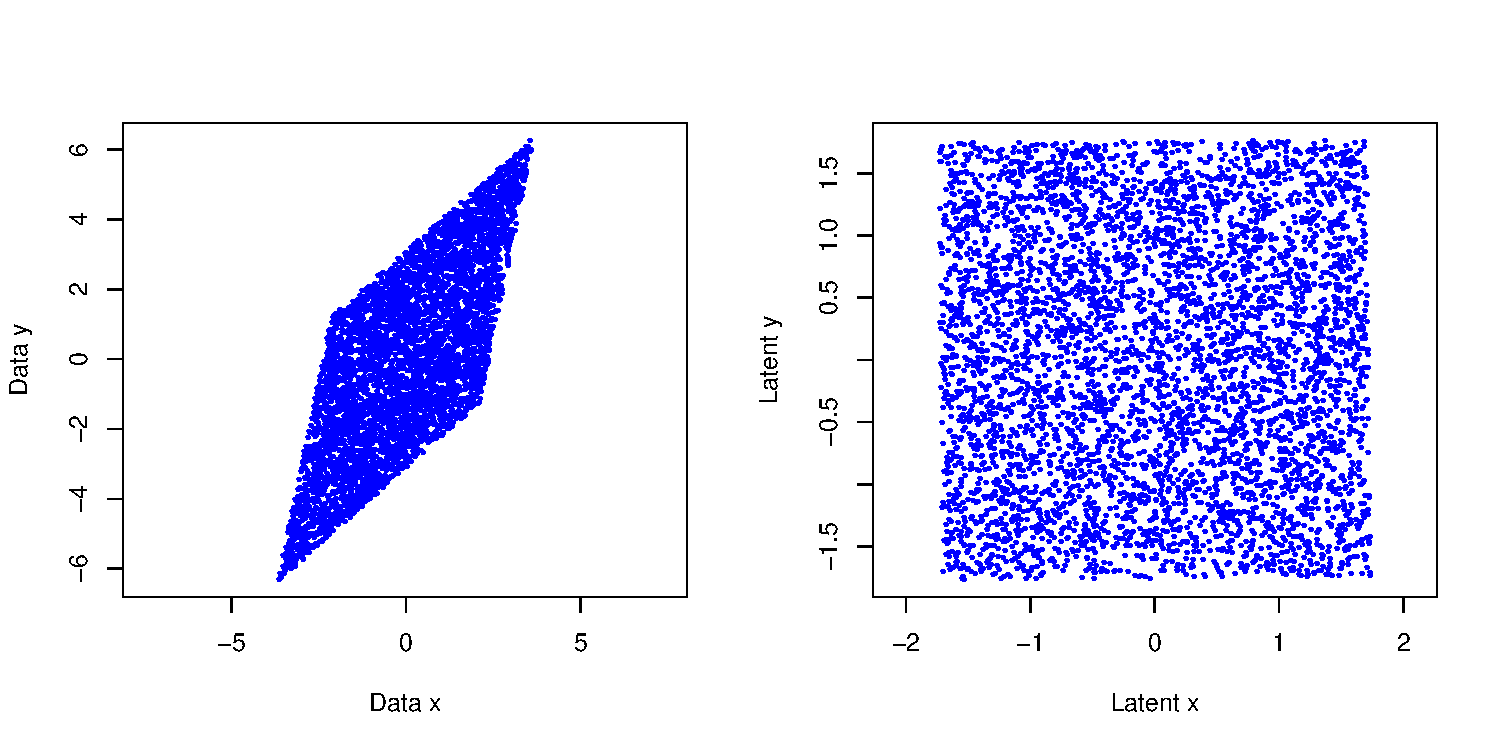
\includegraphics[scale=0.6]{icatest}
	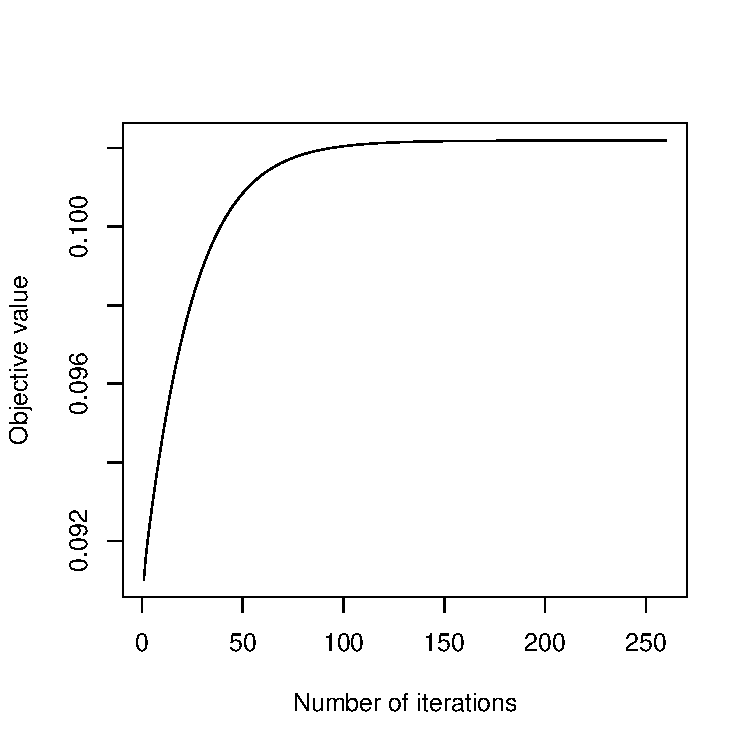
\includegraphics[scale=0.6]{icaobj}
	\caption{Top: the point set \vec{x_1} and the independent components extracted from it.
	Bottom: The convergence of the objective value $F$ while performing ICA on \vec{x_1}.}\label{fig:icatest}
\end{figure}

At the end of the optimization, the final values of $\gamma_i$ are:
\begin{verbatim}
> ica(x1)$gamma
[1] -0.1322905 -0.1221980
\end{verbatim}
The values are negative for both variables, as we could expect because uniform distribution is subgaussian.

\subsection{Exercise 4}

The algorithm was applied to the mixture of images $X$.
The result (with some signs flipped manually) is shown in Figure~\ref{fig:icares}.
The images are very clearly separated in the result.
The colors of some of the images had to be reversed manually, because in the ICA model $\vec x=A\vec s$ it is impossible to measure the signs of $s_i$ from \vec{x} because the signs could get changed in the unknown mixing matrix $A$.
For the same reason we cannot know exactly how dark or light the original images were, so contrast might be wrong in some of the results.

\begin{figure}\centering
	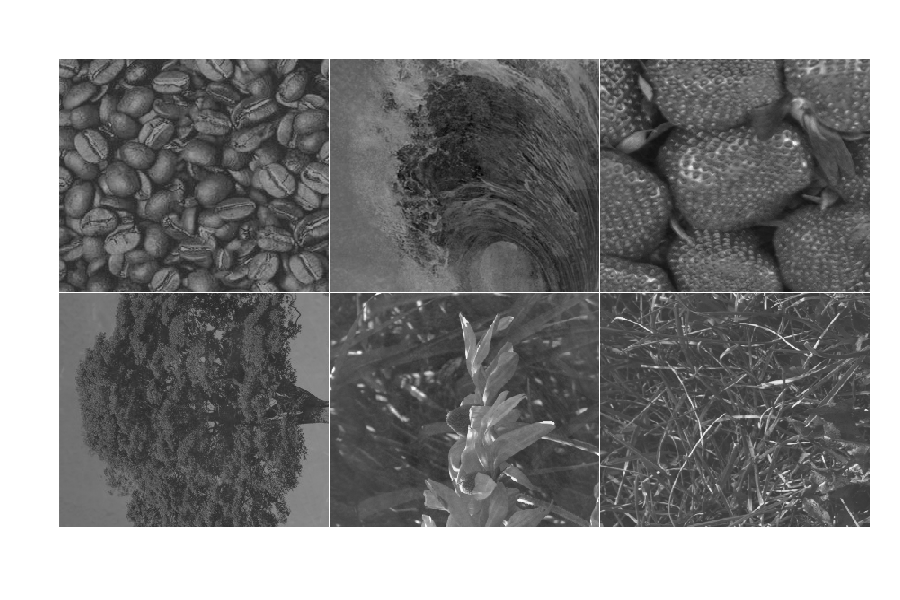
\includegraphics[scale=\iscale]{icares}
	\caption{Result of performing ICA on the whitened mixtures of images.
	As the signs of the latent variables cannot be estimated from the mixtures, some of the images were multiplied manually by -1.}\label{fig:icares}
\end{figure}

At the end of the optimization, for the variables $\gamma_i$ we obtain:
\begin{verbatim}
> ica_result$gamma
[1] -0.08571442 -0.10709199 0.04650270  -0.11421166  0.14818749  0.19895902
\end{verbatim}
The values give a measure on the distribution of the shades of gray in the images.
Supergaussian random variables have a peaked distribution whereas subgaussian ones have more uniform and flat distribution.
Thus the leftmost images and the top-middle image of Figure~\ref{fig:icares} contain all shades fairly uniformly, whereas for the others the distribution is more uneven.


\end{document}
